\begin{figure}[htbp]
    \centering
    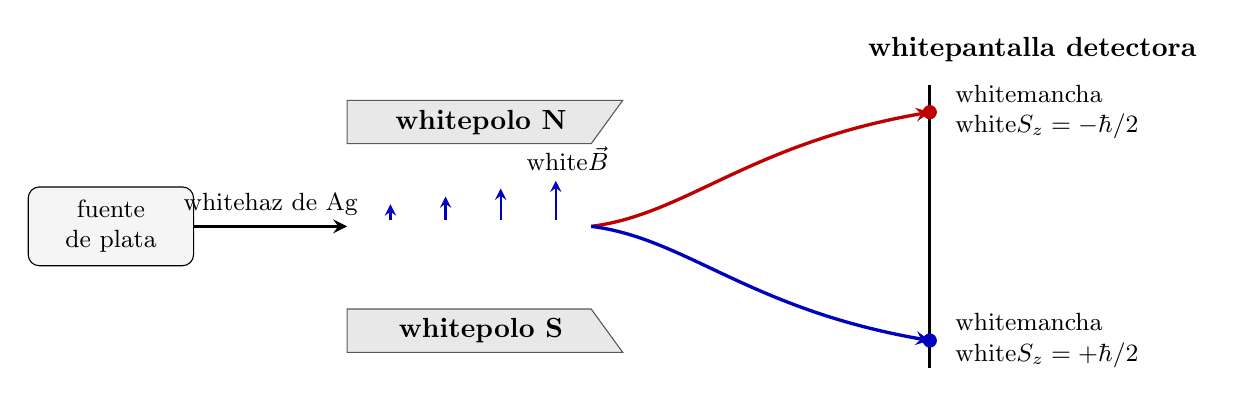
\begin{tikzpicture}[>=stealth, every node/.style={font=\small}]
        \node[draw,rounded corners,fill=gray!8,minimum width=2.1cm,minimum height=1cm,align=center] (source) at (1.0,0) {fuente\\de plata};
        \draw[->,very thick] (source.east) -- (4.0,0) node[midway,above] {\contour{white}{haz de Ag}};

        \draw[fill=gray!18,draw=gray!70!black] (4.0,1.6) -- (7.5,1.6) -- (7.1,1.05) -- (4.0,1.05) -- cycle;
        \draw[fill=gray!18,draw=gray!70!black] (4.0,-1.05) -- (7.1,-1.05) -- (7.5,-1.6) -- (4.0,-1.6) -- cycle;
        \node[font=\bfseries] at (5.7,1.32) {\contour{white}{polo N}};
        \node[font=\bfseries] at (5.7,-1.32) {\contour{white}{polo S}};
        \foreach \x/\h in {4.55/0.28,5.25/0.38,5.95/0.48,6.65/0.58} {
            \draw[->,blue!75!black,thick] (\x,0.08) -- (\x,\h);
        }
        \node[above] at (6.8,0.58) {\contour{white}{$\vec{B}$}};

        \draw[->,very thick,red!75!black] (7.1,0) .. controls (8.3,0.15) and (9.1,1.05) .. (11.4,1.45);
        \draw[->,very thick,blue!75!black] (7.1,0) .. controls (8.3,-0.15) and (9.1,-1.05) .. (11.4,-1.45);

        \draw[very thick] (11.4,-1.8) -- (11.4,1.8);
        \fill[red!75!black] (11.4,1.45) circle (0.09);
        \fill[blue!75!black] (11.4,-1.45) circle (0.09);
        \node[right,align=left] at (11.6,1.45) {\contour{white}{mancha}\\\contour{white}{$S_z=-\hbar/2$}};
        \node[right,align=left] at (11.6,-1.45) {\contour{white}{mancha}\\\contour{white}{$S_z=+\hbar/2$}};
        \node[font=\bfseries] at (12.7,2.25) {\contour{white}{pantalla detectora}};
    \end{tikzpicture}
    \caption{Esquema del experimento de Stern--Gerlach para átomos de plata en un campo inhomogéneo, con $\vec{B}=B_z\vec{e}_z$ y $\partial B_z/\partial z>0$. La fuerza es $\vec{F}=\mu_z(\partial B_z/\partial z)\vec{e}_z$; como el momento magnético del electrón $\vec{\mu}_e=-g_e\mu_B\vec{S}/\hbar$ es antiparalelo a su espín, los estados $S_z=\pm\hbar/2$ se desvían en sentidos opuestos.}
    \label{fig:sg-apparatus}
\end{figure}